% Options for packages loaded elsewhere
\PassOptionsToPackage{unicode}{hyperref}
\PassOptionsToPackage{hyphens}{url}
%
\documentclass[
]{ltjarticle}
\usepackage{lmodern}
\usepackage{amssymb,amsmath}
\usepackage{ifxetex,ifluatex}
\ifnum 0\ifxetex 1\fi\ifluatex 1\fi=0 % if pdftex
  \usepackage[T1]{fontenc}
  \usepackage[utf8]{inputenc}
  \usepackage{textcomp} % provide euro and other symbols
\else % if luatex or xetex
  \usepackage{unicode-math}
  \defaultfontfeatures{Scale=MatchLowercase}
  \defaultfontfeatures[\rmfamily]{Ligatures=TeX,Scale=1}
\fi
% Use upquote if available, for straight quotes in verbatim environments
\IfFileExists{upquote.sty}{\usepackage{upquote}}{}
\IfFileExists{microtype.sty}{% use microtype if available
  \usepackage[]{microtype}
  \UseMicrotypeSet[protrusion]{basicmath} % disable protrusion for tt fonts
}{}
\makeatletter
\@ifundefined{KOMAClassName}{% if non-KOMA class
  \IfFileExists{parskip.sty}{%
    \usepackage{parskip}
  }{% else
    \setlength{\parindent}{0pt}
    \setlength{\parskip}{6pt plus 2pt minus 1pt}}
}{% if KOMA class
  \KOMAoptions{parskip=half}}
\makeatother
\usepackage{xcolor}
\IfFileExists{xurl.sty}{\usepackage{xurl}}{} % add URL line breaks if available
\IfFileExists{bookmark.sty}{\usepackage{bookmark}}{\usepackage{hyperref}}
\hypersetup{
  pdftitle={Summary of Data Structures},
  pdfauthor={Jake Underland (1A193008-2)},
  hidelinks,
  pdfcreator={LaTeX via pandoc}}
\urlstyle{same} % disable monospaced font for URLs
\usepackage[margin=2cm]{geometry}
\usepackage{color}
\usepackage{fancyvrb}
\newcommand{\VerbBar}{|}
\newcommand{\VERB}{\Verb[commandchars=\\\{\}]}
\DefineVerbatimEnvironment{Highlighting}{Verbatim}{commandchars=\\\{\}}
% Add ',fontsize=\small' for more characters per line
\usepackage{framed}
\definecolor{shadecolor}{RGB}{248,248,248}
\newenvironment{Shaded}{\begin{snugshade}}{\end{snugshade}}
\newcommand{\AlertTok}[1]{\textcolor[rgb]{0.94,0.16,0.16}{#1}}
\newcommand{\AnnotationTok}[1]{\textcolor[rgb]{0.56,0.35,0.01}{\textbf{\textit{#1}}}}
\newcommand{\AttributeTok}[1]{\textcolor[rgb]{0.77,0.63,0.00}{#1}}
\newcommand{\BaseNTok}[1]{\textcolor[rgb]{0.00,0.00,0.81}{#1}}
\newcommand{\BuiltInTok}[1]{#1}
\newcommand{\CharTok}[1]{\textcolor[rgb]{0.31,0.60,0.02}{#1}}
\newcommand{\CommentTok}[1]{\textcolor[rgb]{0.56,0.35,0.01}{\textit{#1}}}
\newcommand{\CommentVarTok}[1]{\textcolor[rgb]{0.56,0.35,0.01}{\textbf{\textit{#1}}}}
\newcommand{\ConstantTok}[1]{\textcolor[rgb]{0.00,0.00,0.00}{#1}}
\newcommand{\ControlFlowTok}[1]{\textcolor[rgb]{0.13,0.29,0.53}{\textbf{#1}}}
\newcommand{\DataTypeTok}[1]{\textcolor[rgb]{0.13,0.29,0.53}{#1}}
\newcommand{\DecValTok}[1]{\textcolor[rgb]{0.00,0.00,0.81}{#1}}
\newcommand{\DocumentationTok}[1]{\textcolor[rgb]{0.56,0.35,0.01}{\textbf{\textit{#1}}}}
\newcommand{\ErrorTok}[1]{\textcolor[rgb]{0.64,0.00,0.00}{\textbf{#1}}}
\newcommand{\ExtensionTok}[1]{#1}
\newcommand{\FloatTok}[1]{\textcolor[rgb]{0.00,0.00,0.81}{#1}}
\newcommand{\FunctionTok}[1]{\textcolor[rgb]{0.00,0.00,0.00}{#1}}
\newcommand{\ImportTok}[1]{#1}
\newcommand{\InformationTok}[1]{\textcolor[rgb]{0.56,0.35,0.01}{\textbf{\textit{#1}}}}
\newcommand{\KeywordTok}[1]{\textcolor[rgb]{0.13,0.29,0.53}{\textbf{#1}}}
\newcommand{\NormalTok}[1]{#1}
\newcommand{\OperatorTok}[1]{\textcolor[rgb]{0.81,0.36,0.00}{\textbf{#1}}}
\newcommand{\OtherTok}[1]{\textcolor[rgb]{0.56,0.35,0.01}{#1}}
\newcommand{\PreprocessorTok}[1]{\textcolor[rgb]{0.56,0.35,0.01}{\textit{#1}}}
\newcommand{\RegionMarkerTok}[1]{#1}
\newcommand{\SpecialCharTok}[1]{\textcolor[rgb]{0.00,0.00,0.00}{#1}}
\newcommand{\SpecialStringTok}[1]{\textcolor[rgb]{0.31,0.60,0.02}{#1}}
\newcommand{\StringTok}[1]{\textcolor[rgb]{0.31,0.60,0.02}{#1}}
\newcommand{\VariableTok}[1]{\textcolor[rgb]{0.00,0.00,0.00}{#1}}
\newcommand{\VerbatimStringTok}[1]{\textcolor[rgb]{0.31,0.60,0.02}{#1}}
\newcommand{\WarningTok}[1]{\textcolor[rgb]{0.56,0.35,0.01}{\textbf{\textit{#1}}}}
\usepackage{longtable,booktabs}
% Correct order of tables after \paragraph or \subparagraph
\usepackage{etoolbox}
\makeatletter
\patchcmd\longtable{\par}{\if@noskipsec\mbox{}\fi\par}{}{}
\makeatother
% Allow footnotes in longtable head/foot
\IfFileExists{footnotehyper.sty}{\usepackage{footnotehyper}}{\usepackage{footnote}}
\makesavenoteenv{longtable}
\usepackage{graphicx,grffile}
\makeatletter
\def\maxwidth{\ifdim\Gin@nat@width>\linewidth\linewidth\else\Gin@nat@width\fi}
\def\maxheight{\ifdim\Gin@nat@height>\textheight\textheight\else\Gin@nat@height\fi}
\makeatother
% Scale images if necessary, so that they will not overflow the page
% margins by default, and it is still possible to overwrite the defaults
% using explicit options in \includegraphics[width, height, ...]{}
\setkeys{Gin}{width=\maxwidth,height=\maxheight,keepaspectratio}
% Set default figure placement to htbp
\makeatletter
\def\fps@figure{htbp}
\makeatother
\setlength{\emergencystretch}{3em} % prevent overfull lines
\providecommand{\tightlist}{%
  \setlength{\itemsep}{0pt}\setlength{\parskip}{0pt}}
\setcounter{secnumdepth}{5}
\usepackage{graphicx}
\graphicspath{ {images/} }
\usepackage{subfig}
\usepackage{enumitem}
\hypersetup{ filecolor=magenta, urlcolor=cyan, }
\usepackage{forest}
\usepackage{tikz}
\tikzset{ heap/.style={ every node/.style={circle,draw}, level 1/.style={sibling distance=30mm}, level 2/.style={sibling distance=10mm} } }
\usepackage{amsmath}
\usepackage{color}
\usepackage{hyperref}
\usepackage{luatexja}

\title{Summary of Data Structures}
\author{Jake Underland (1A193008-2)}
\date{1/30/2022}

\begin{document}
\maketitle

{
\setcounter{tocdepth}{3}
\tableofcontents
}
\begin{abstract} 
本レポートではkd木,フィボナッチヒープ,AVL木,接尾辞配列の4つのデータ構造について解説していく.
\end{abstract}

\hypertarget{k-dux6728}{%
\section{k-d木}\label{k-dux6728}}

\(k\)-d木とは,二分木の一つであり,全てのノードが\(k\)次元のユークリッド空間上の点であるものをいう.二分木であるため,全てのノードには2つの子供ノード(左,右)がある.\(k\)次元の座標空間のいずれかの軸(例:2次元空間の\(x\)軸)に着目し,根ノードの軸の値と新しく挿入するノードの軸の値を比較して挿入するノードの方が低ければ,根ノードの左部分木に挿入し,高ければ,根ノードの右部分木に挿入する.これを,親から辿っていき全てのノードを部分木とみなして再帰的に行うことで挿入することができる.一般的には,深さが増すごとに基準となる軸を交互に変えていく.これが意味することは,すなわち全ての葉ではないノードは,座標空間を2つの半空間に分割する超平面を作り出しており,そのノードの下に属するノードは2つに仕分けられる.ここまでのロジックを組んだコードをpythonで実装してみたのが以下だ.

\begin{Shaded}
\begin{Highlighting}[]
\KeywordTok{class}\NormalTok{ kdtree(}\BuiltInTok{object}\NormalTok{):}
    \KeywordTok{def} \FunctionTok{__init__}\NormalTok{(}\VariableTok{self}\NormalTok{, point, axis}\OperatorTok{=}\DecValTok{0}\NormalTok{):}
        \VariableTok{self}\NormalTok{.point }\OperatorTok{=}\NormalTok{ point }\CommentTok{# k次元の座標(tuple)}
        \VariableTok{self}\NormalTok{.k }\OperatorTok{=} \BuiltInTok{len}\NormalTok{(}\VariableTok{self}\NormalTok{.point)}
        \VariableTok{self}\NormalTok{.axis }\OperatorTok{=}\NormalTok{ axis }\OperatorTok{%} \VariableTok{self}\NormalTok{.k  }\CommentTok{# 比較する軸をincrement することで交互に入れ替える}
        \VariableTok{self}\NormalTok{.left_child }\OperatorTok{=} \VariableTok{None}
        \VariableTok{self}\NormalTok{.right_child }\OperatorTok{=} \VariableTok{None}
        \VariableTok{self}\NormalTok{.children }\OperatorTok{=}\NormalTok{ []}
    
    \KeywordTok{def}\NormalTok{ insert(}\VariableTok{self}\NormalTok{, point):}
        \ControlFlowTok{assert} \BuiltInTok{len}\NormalTok{(point) }\OperatorTok{==} \VariableTok{self}\NormalTok{.k}
        \ControlFlowTok{if}\NormalTok{ point[}\VariableTok{self}\NormalTok{.axis] }\OperatorTok{>} \VariableTok{self}\NormalTok{.point[}\VariableTok{self}\NormalTok{.axis]:}
            \ControlFlowTok{if} \VariableTok{self}\NormalTok{.right_child:}
                \VariableTok{self}\NormalTok{.right_child.insert(point)}
            \ControlFlowTok{else}\NormalTok{:}
                \VariableTok{self}\NormalTok{.right_child }\OperatorTok{=}\NormalTok{ kdtree(point, }\VariableTok{self}\NormalTok{.axis }\OperatorTok{+} \DecValTok{1}\NormalTok{)}
                \VariableTok{self}\NormalTok{.children.insert(}\DecValTok{0}\NormalTok{, }\VariableTok{self}\NormalTok{.right_child)}
        \ControlFlowTok{else}\NormalTok{:}
            \ControlFlowTok{if} \VariableTok{self}\NormalTok{.left_child:}
                \VariableTok{self}\NormalTok{.left_child.insert(point)}
            \ControlFlowTok{else}\NormalTok{:}
                \VariableTok{self}\NormalTok{.left_child }\OperatorTok{=}\NormalTok{ kdtree(point, }\VariableTok{self}\NormalTok{.axis }\OperatorTok{+} \DecValTok{1}\NormalTok{)}
                \VariableTok{self}\NormalTok{.children.append(}\VariableTok{self}\NormalTok{.left_child)}
\end{Highlighting}
\end{Shaded}

これを可視化したのが以下になる.ただし,ターミナルでの可視化の都合上,右の子ノードを上,左の子ノードが下に来るように,木全体を左方向に90度傾けた様子となっている.

\begin{figure}
\centering
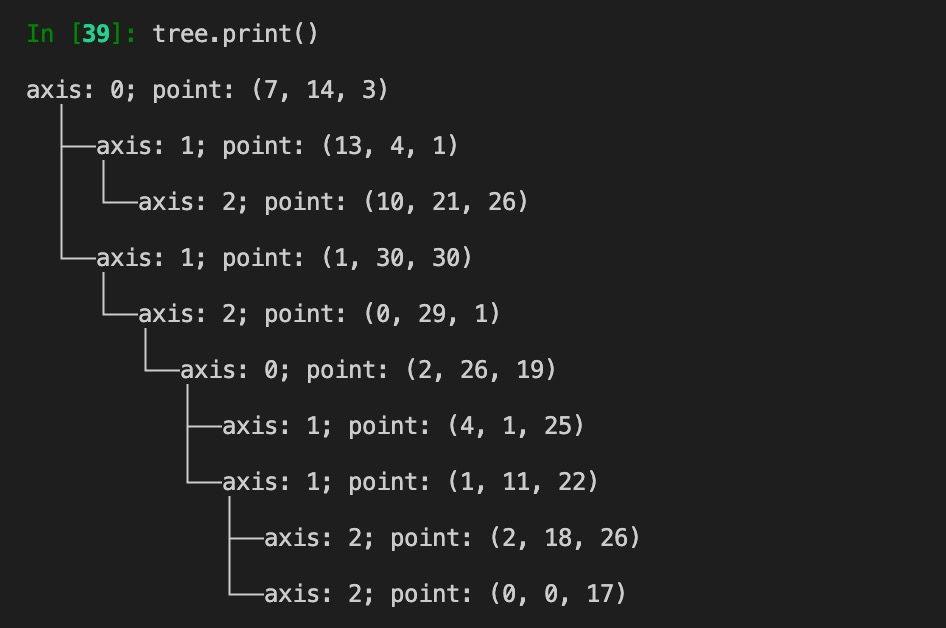
\includegraphics[width=0.7\textwidth]{kdtree.jpg}
\end{figure}

\texttt{axis}が参照される座標軸を指し,深度が増すごとに入れ替わっているのが観察できる.また,全てのノードにおいて,その下に属するノードは,指定された座標軸で2つの半空間に分割されていることが見て取れる.

kd
木は多次元データを扱う際に有用である.例えば,簡略化のため,下の2次元のkd木に注目する.

\begin{figure}
\centering
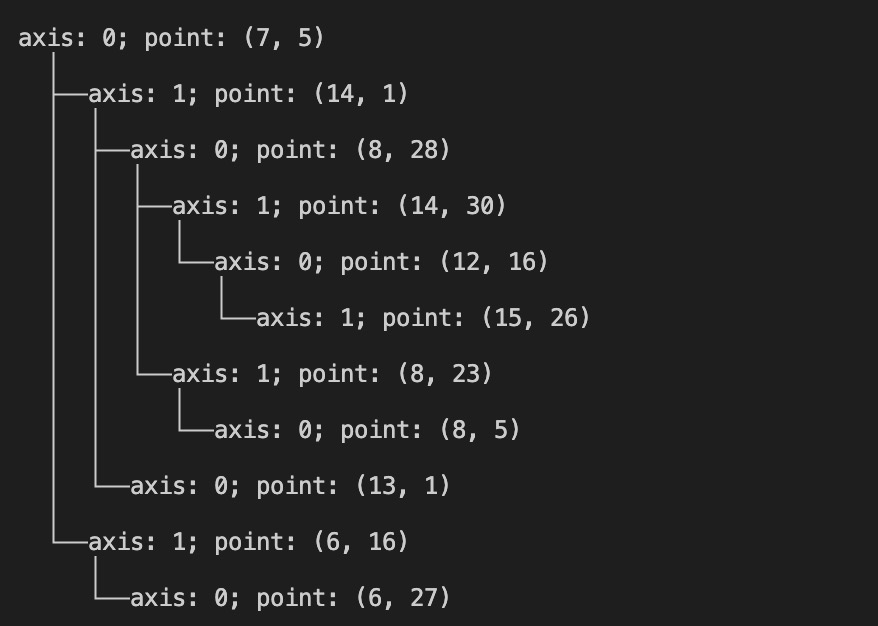
\includegraphics[width=0.7\textwidth]{tree2.jpg}
\end{figure}

\texttt{(14,\ 23)}
に最も近い(ユークリッド距離が最小な)点を探したいとする.この時,根っこからkd木を辿ってみる.\(14 >7\)なので,右の(上の)部分木に移る.\(23 > 1\)なので,また右の部分木に移る.この移動を繰り返すたびに,探索する範囲は狭くなっていき,最終的に直近点の近傍に落ち着き,その範囲内の点を探すことにより直近点を割り出すことができる.このような繰り返した領域のパーテーションがkd木の特徴である.したの図は,2次元空間におけるこのパーテーションの反復を可視化したものだ.

\begin{figure}
\centering
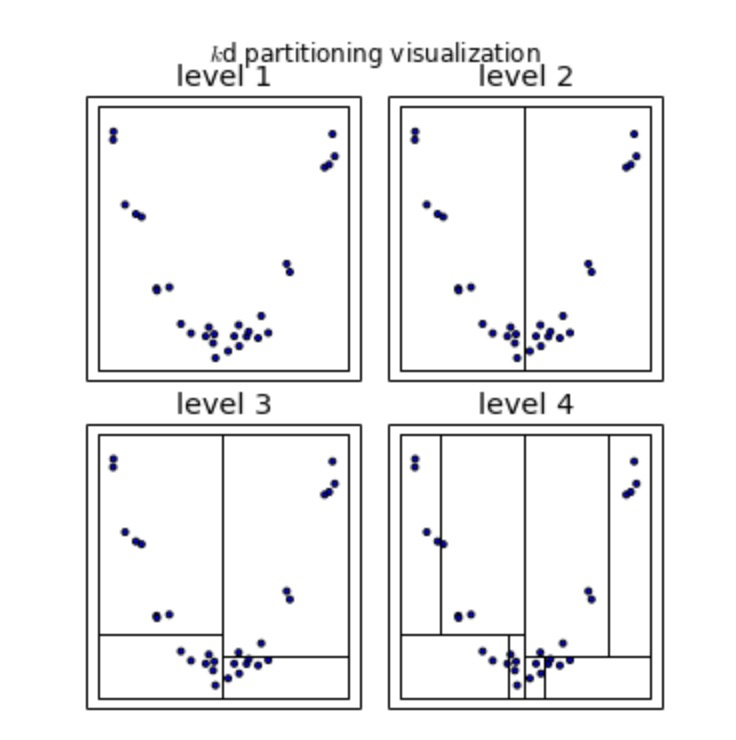
\includegraphics[width=0.7\textwidth]{partition.jpg}
\end{figure}

\newpage

\hypertarget{ux30d5ux30a3ux30dcux30caux30c3ux30c1ux30d2ux30fcux30d7}{%
\section{フィボナッチヒープ}\label{ux30d5ux30a3ux30dcux30caux30c3ux30c1ux30d2ux30fcux30d7}}

フィボナッチヒープとは,マージ可能なヒープ構造をしており,以下の操作を行うことができる:

\begin{itemize}
\item ヒープ作成:ヒープを作る  
\item 挿入:ヒープに追加する  
\item 最小値:ヒープの中の最小値へのポインターをリターンする  
\item 最小値抽出:ヒープの中の最小値へのポインターをリターンし,最小値をヒープから削除する  
\item マージ:二つのヒープをマージする  
\item 要素の下方更新:ヒープのある要素の値を,それ以下の値に更新する  
\item 削除:ヒープから要素を削除する. 
\end{itemize}

フィボナッチヒープの利点としては,これらの操作のうちの多くを定数時間で行うことができることだ.二分ヒープと比較すると以下のようになる.

\begin{longtable}[]{@{}lll@{}}
\toprule
& 二分ヒープ & フィボナッチヒープ\tabularnewline
\midrule
\endhead
ヒープ作成 & \(O(1)\) & \(O(1)\)\tabularnewline
挿入 & \(O(\log n)\) & \(O(1)\)\tabularnewline
最小値 & \(O(1)\) & \(O(1)\)\tabularnewline
最小値抽出 & \(O(\log n)\) & \(O(\log n)\)\tabularnewline
マージ & \(O(n)\) & \(O(1)\)\tabularnewline
要素の下方更新 & \(O(\log n)\) & \(O(1)\)\tabularnewline
削除 & \(O(\log n)\) & \(O(\log n)\)\tabularnewline
\bottomrule
\end{longtable}

フィボナッチヒープの構造は,最小ヒープの性質(子ノードの方が親ノードより値が大きい)を持った木の集合である.二項ヒープと違い,この集合にの木の形に規定はなく,また同じ形をした木が複数あっても構わない.そのため,木のマージや挿入は,単純に木をつなぎ合わせれば完了する.これがこれらの操作の高速化の理由である.また,要素の下方更新はその要素を独立の木として切り離して行われることもあるため,この操作も高速化される.

\begin{figure}
\centering
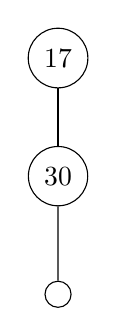
\begin{tikzpicture}[heap]
  \node {17}
  child{node{30}
    child{node{}}
  }
  ;
\end{tikzpicture}
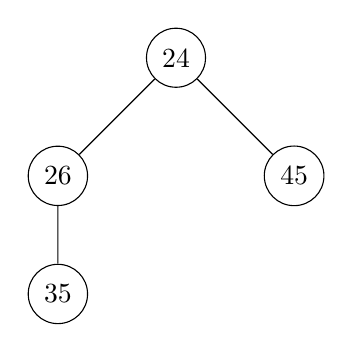
\begin{tikzpicture}[heap]
  \node {24}
  child{node{26}
    child{node{35}}}
  child{node{45}}
  ;
\end{tikzpicture}
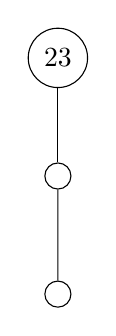
\begin{tikzpicture}[heap]
  \node {23}
    child{node{}
      child{node{}}
  }
  ;
\end{tikzpicture}
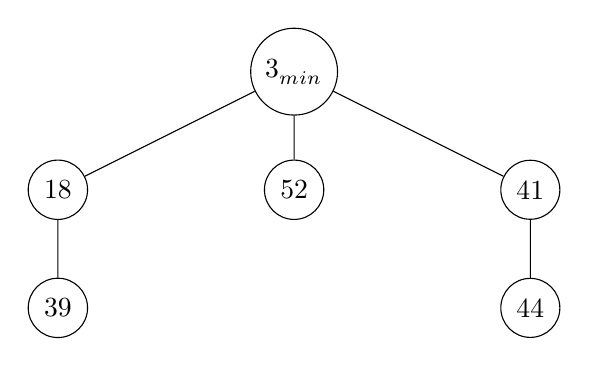
\begin{tikzpicture}[heap]
  \node {$3_{min}$}
  child{node{18}
    child{node{39}}}
  child{node{52}}
  child{node{41}
    child{node{44}}}
  ;
\end{tikzpicture}
\caption{フィボナッチヒープ(但し空のノードは高さを揃えるためのもの).}
\end{figure}

フィボナッチヒープは最小値を示すポインターの情報を保存しており,ヒープ内の全ての木の最小値が連結リスト(双方向循環リスト)によりつながっているため,一つのポインターで全ての木の最小値をアクセスすることができる.図2では描かれていないが,根のノードは全て連結されている.

フィボナッチヒープで最も複雑な操作は最小値の抽出と削除である.最小値の抽出は,以下のように進む:\\

\begin{enumerate}
\item 最小ノードを削除する  
\item 削除したノードの部分木の根を全て根の連結リストに加え,最小のものを先頭に持ってくる.
\item 根のリスト上で次元が等しい木をマージする(二項ヒープと同様).これを,全ての木の次元が異なるまで続ける.  
\item 残った根の中から最小値を見つけ,ポインターを指す. 
\end{enumerate}

\begin{figure}
\centering
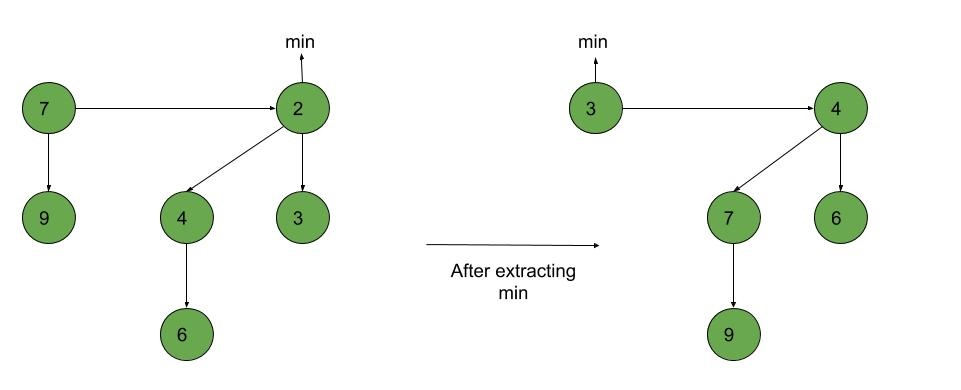
\includegraphics[width=0.7\textwidth]{fib-heap-extr-min-1.jpg}
\caption{\href{https://www.geeksforgeeks.org/fibonacci-heap-deletion-extract-min-and-decrease-key/}{最小値抽出}}
\end{figure}

削除操作は削除する要素の値を\(-\infty\)に更新してから上の操作を行えばいい.

フィボナッチヒープはヒープのマージ,挿入,下方更新を多く行う必要があるアルゴリズムによく使われる.

\newpage

\hypertarget{avlux6728}{%
\section{AVL木}\label{avlux6728}}

AVL木とは二分探索木の一種で,どのノードの左右部分木の高さも差が1以内のものを指す.このような条件を満たす木を平衡二分探索木というが,AVLには,何らかの操作によってどこかで左右部分木の高さに1を超える差が生じても,再び平衡となるように自身を再構成できることが特徴である.

通常の2分探索木は,それぞれの頂点が最高2つの子を持つ二分木で,次の特徴を満たす:\\
全ての頂点\texttt{v}において,\texttt{v}の左部分木に含まれるどの頂点\texttt{v\_l}に対しても\texttt{v.key()\ \textgreater{}=\ v\_l.key()}であり,\texttt{v}の右部分木に含まれるどの頂点\texttt{v\_r}にたいしても\texttt{v.key()\ \textless{}=\ v\_r.key()}が成り立つ.

この性質の結果,二分探索木の構造は要素を挿入する順序に大きく依存する(図3参照).

\begin{figure}%
    \centering
    \subfloat[\centering 一般的な二分探索木]{{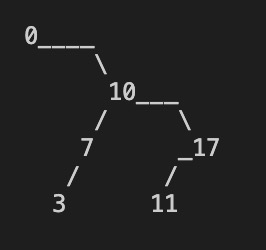
\includegraphics[width=0.45\textwidth]{bst.jpg} }}%
    \qquad
    \subfloat[\centering ソートされた順に挿入した時の二分探索木]{{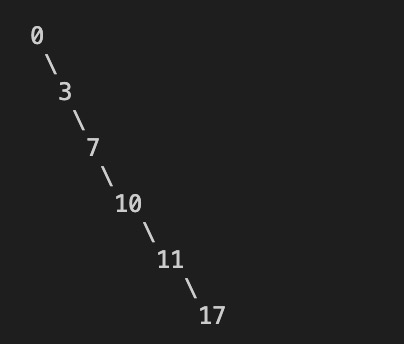
\includegraphics[width=0.45\textwidth]{sorted_bst.jpg} }}%
    \caption{同じ整数の集合でも,挿入の順序で木の形が大きく変わる.}
    %\label{fig:example}%
\end{figure}

バランスが比較的保たれた二分探索木では,\(2^h = N\)であり,なお二分探索木への操作のほとんどは\(O(h)\)なので,結果\(O(\log N)\)となるしかし,図3の(b)の場合は,\(h=N\)となっているため,操作の計算量は\(O(N)\)と大きく増加する.

この問題を,AVL木は解消する.AVL木は,削除,挿入といった操作の後に,必ず右部分木の高さと左部分木の高さの差を確認する.差が1を超えるようであれば,木は回転を行う.木の回転には右回転と左回転があり,それぞれは要素の順番を崩さずに右回転であれば右部分木の高さを1増やして左部分木の高さを1減らし,左回転であれば左部分木の高さを1増やして右部分木の高さを1減らす.その様子は,下の図に表される

\begin{figure}
\centering
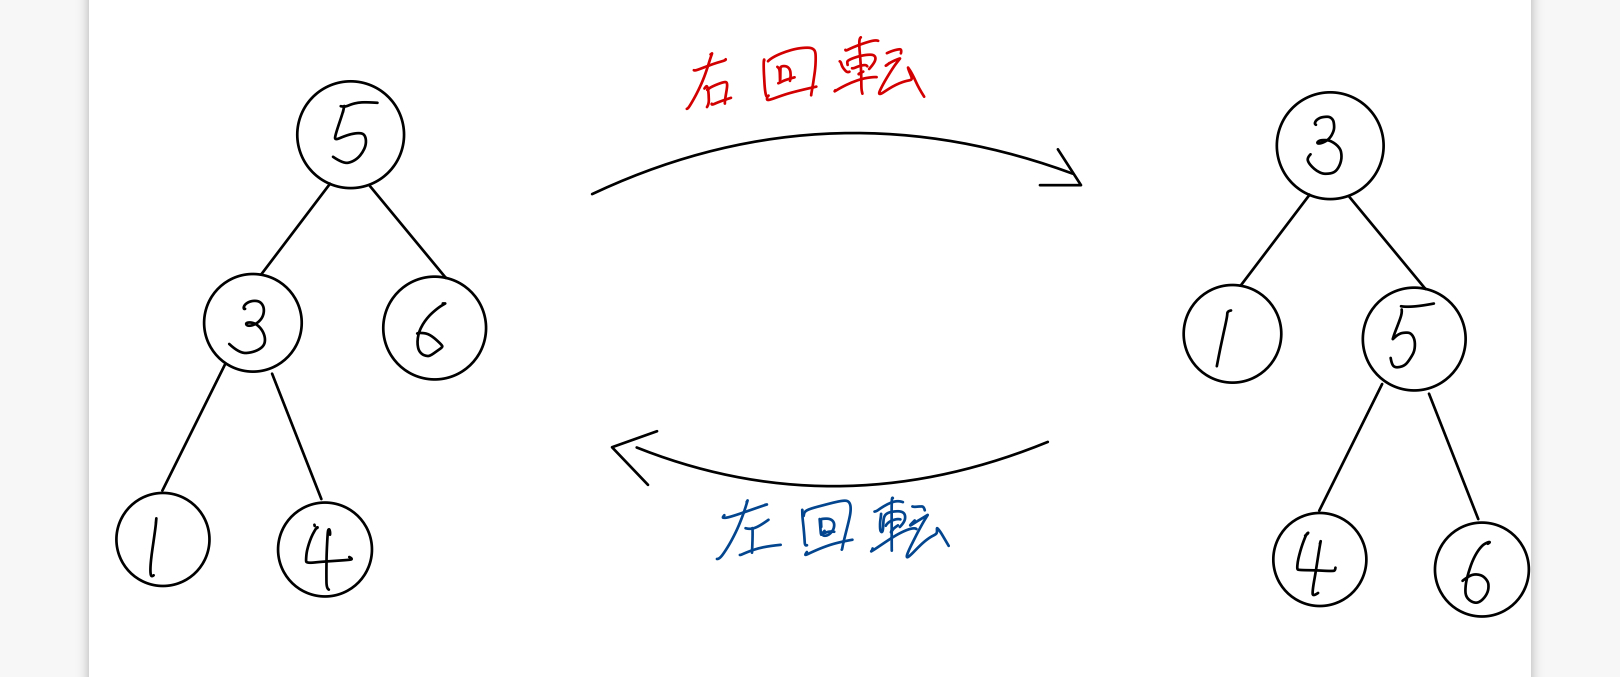
\includegraphics[width=0.7\textwidth]{rotate.jpeg}
\end{figure}

AVL木は回転を通して常に平衡であるため,確実に\(O(\log N)\)に近い計算量で操作を実現している.

\newpage

\hypertarget{ux63a5ux5c3eux8f9eux914dux5217}{%
\section{接尾辞配列}\label{ux63a5ux5c3eux8f9eux914dux5217}}

接尾辞配列とは,ある文字列の接尾辞を全て抽出し,それをアルファベット順に並べた時の,各接尾辞の位置を保存した配列である.以下のコードは,pythonでこれを実装したものである.

\begin{Shaded}
\begin{Highlighting}[]
\KeywordTok{def}\NormalTok{ extract_suffix_array(string):}
\NormalTok{    n }\OperatorTok{=} \BuiltInTok{len}\NormalTok{(string)}
\NormalTok{    suffixes }\OperatorTok{=}\NormalTok{ []}
    \ControlFlowTok{for}\NormalTok{ i }\KeywordTok{in} \BuiltInTok{range}\NormalTok{(n):}
\NormalTok{        suffixes.append((i, string[i:]))}
\NormalTok{    sorted_suffixes }\OperatorTok{=} \BuiltInTok{sorted}\NormalTok{(suffixes, key}\OperatorTok{=}\KeywordTok{lambda}\NormalTok{ x:x[}\DecValTok{1}\NormalTok{])}
    \ControlFlowTok{for}\NormalTok{ i }\KeywordTok{in} \BuiltInTok{range}\NormalTok{(n):}
        \BuiltInTok{print}\NormalTok{ suffixes[i], }\StringTok{" "} \OperatorTok{*}\NormalTok{ i, }\StringTok{"   --->  "}\NormalTok{, sorted_suffixes[i]}
    \ControlFlowTok{return}\NormalTok{ [x[}\DecValTok{0}\NormalTok{] }\ControlFlowTok{for}\NormalTok{ x }\KeywordTok{in}\NormalTok{ sorted_suffixes]}

\NormalTok{string }\OperatorTok{=} \StringTok{"algorithms"}
\NormalTok{suffix_array }\OperatorTok{=}\NormalTok{ extract_suffix_array(string)}
\end{Highlighting}
\end{Shaded}

\begin{verbatim}
## (0, 'algorithms')     --->   (0, 'algorithms')
## (1, 'lgorithms')      --->   (2, 'gorithms')
## (2, 'gorithms')       --->   (7, 'hms')
## (3, 'orithms')        --->   (5, 'ithms')
## (4, 'rithms')         --->   (1, 'lgorithms')
## (5, 'ithms')          --->   (8, 'ms')
## (6, 'thms')           --->   (3, 'orithms')
## (7, 'hms')            --->   (4, 'rithms')
## (8, 'ms')             --->   (9, 's')
## (9, 's')              --->   (6, 'thms')
\end{verbatim}

\begin{Shaded}
\begin{Highlighting}[]
\BuiltInTok{print}\NormalTok{(}\StringTok{"suffix array of '}\SpecialCharTok{\{\}}\StringTok{' is: }\SpecialCharTok{\{\}}\StringTok{"}\NormalTok{.}\BuiltInTok{format}\NormalTok{(string, suffix_array))}
\end{Highlighting}
\end{Shaded}

\begin{verbatim}
## suffix array of 'algorithms' is: [0, 2, 7, 5, 1, 8, 3, 4, 9, 6]
\end{verbatim}

接尾辞配列の代表的な応用例としては,文字列の中の部分文字列の出現回数の探索があげられる.接尾辞配列は全ての可能な接尾辞を含んでいるので,この文字列の中で考えられる部分文字列は,必ずいずれかの接尾辞の接頭辞として存在しているはずだ.また,接尾辞配列ではアルファベット順に並んでいるので,該当するような接尾辞は隣り合わせになっているはずである.よって,二分探索法を2回行うこと(接尾辞配列で最初に部分文字列を含む接尾辞と最後に部分文字列を含む接尾辞)で,効率よく目的の部分文字列の出現回数を判断することができる.

\hypertarget{references}{%
\section{References}\label{references}}

\setlength{\parindent}{-0.2in}
\setlength{\leftskip}{0.2in}
\setlength{\parskip}{8pt}

\noindent

Cormen, T.H., Leiserson, C. E., Rivest, R. L., \& Stein, C. (2009).
Introduction to algorithms (3rd ed.). MIT Press.

VanderPlas, J., Ivezic, Z., Connolly, A., Gray, A. (2013). ``Statistics,
Data Mining, and Machine Learning in Astronomy''. Princeton University
Press.

\url{https://qiita.com/flare/items/20439a1db54b367eea70}

\url{https://www.tutorialspoint.com/data_structures_algorithms/avl_tree_algorithm.htm}

\end{document}
